
\section{誤差論}
%\footnote{以下の論文を読んでの意見である\cite{Error_bar_nature,krzywinski2013importance}}
誤差論は、計測に対する信頼性を定量的に扱う方法論である。
%真である理論値へ実験が近づけたことを検証することを目的にしており、理論に重点をおき、計測を疑うという点で生物学などのデータ解析とは異なる。

\subsection{標準偏差か標準誤差か}
標準偏差や標準誤差によりデータのばらつきを捉えようとすることは、正規分布を含んだモデルを使って、母集団を推測しようとする行為であると考えることができます。以下の議論は、モデルが現象をよく捉えている場合にはうまく成り立つが、そうでないなら、モデルを修正したほうが、うまく現象をうまく捉えることができる\footnote{様々な意見がある\cite{SUZUKI_SESD,池田郁男2013統計検定を理解せずに使っている人のために,池田郁男2019改訂増補版}}。
ここでは、次のモデル$M(\mu,\sigma^2)$を使う。

\begin{enumerate}
    \item i.i.d
    \item 正規分布関数
    \item $\mu,\sigma^2$
\end{enumerate}
ここで、母集団から無作為抽出した標本の標本平均と標本分散をそれぞれ、$\bar{x}=\frac{1}{n}\sum{x_i},s^2=\frac{1}{n}\sum(x_i-\bar{x})^2$である。これらを組み入れた統計モデルを$M(\bar{X},s^2)$と書く。

\subsubsection{標準偏差}
正規分布を含んだ統計モデルを仮定し、そのモデルの上で、予想されるサンプルがおよそ$68\%$の確率で出現する範囲は、母数分散$\sigma^2$より以下の範囲になります。
\begin{equation*}
    [\mu-\sigma,\mu+\sigma].
\end{equation*}
モデルの母数分散は不明な場合、母集団から無作為抽出を行なって集計した標本の偏差$s$を計算します。
\begin{equation*}
    s = \sqrt{\frac{1}{n}\sum(x_i-\bar{x})^2}.
\end{equation*}
このことから、モデルが予測するサンプルが$68\%$の確率で出現する範囲は
\begin{equation*}
    [\mu-s,\mu+s].
\end{equation*}
これを図示したものが、図です。
言い換えれば、これは、$68\%$予測区間である。


\begin{figure}
    \begin{center}
        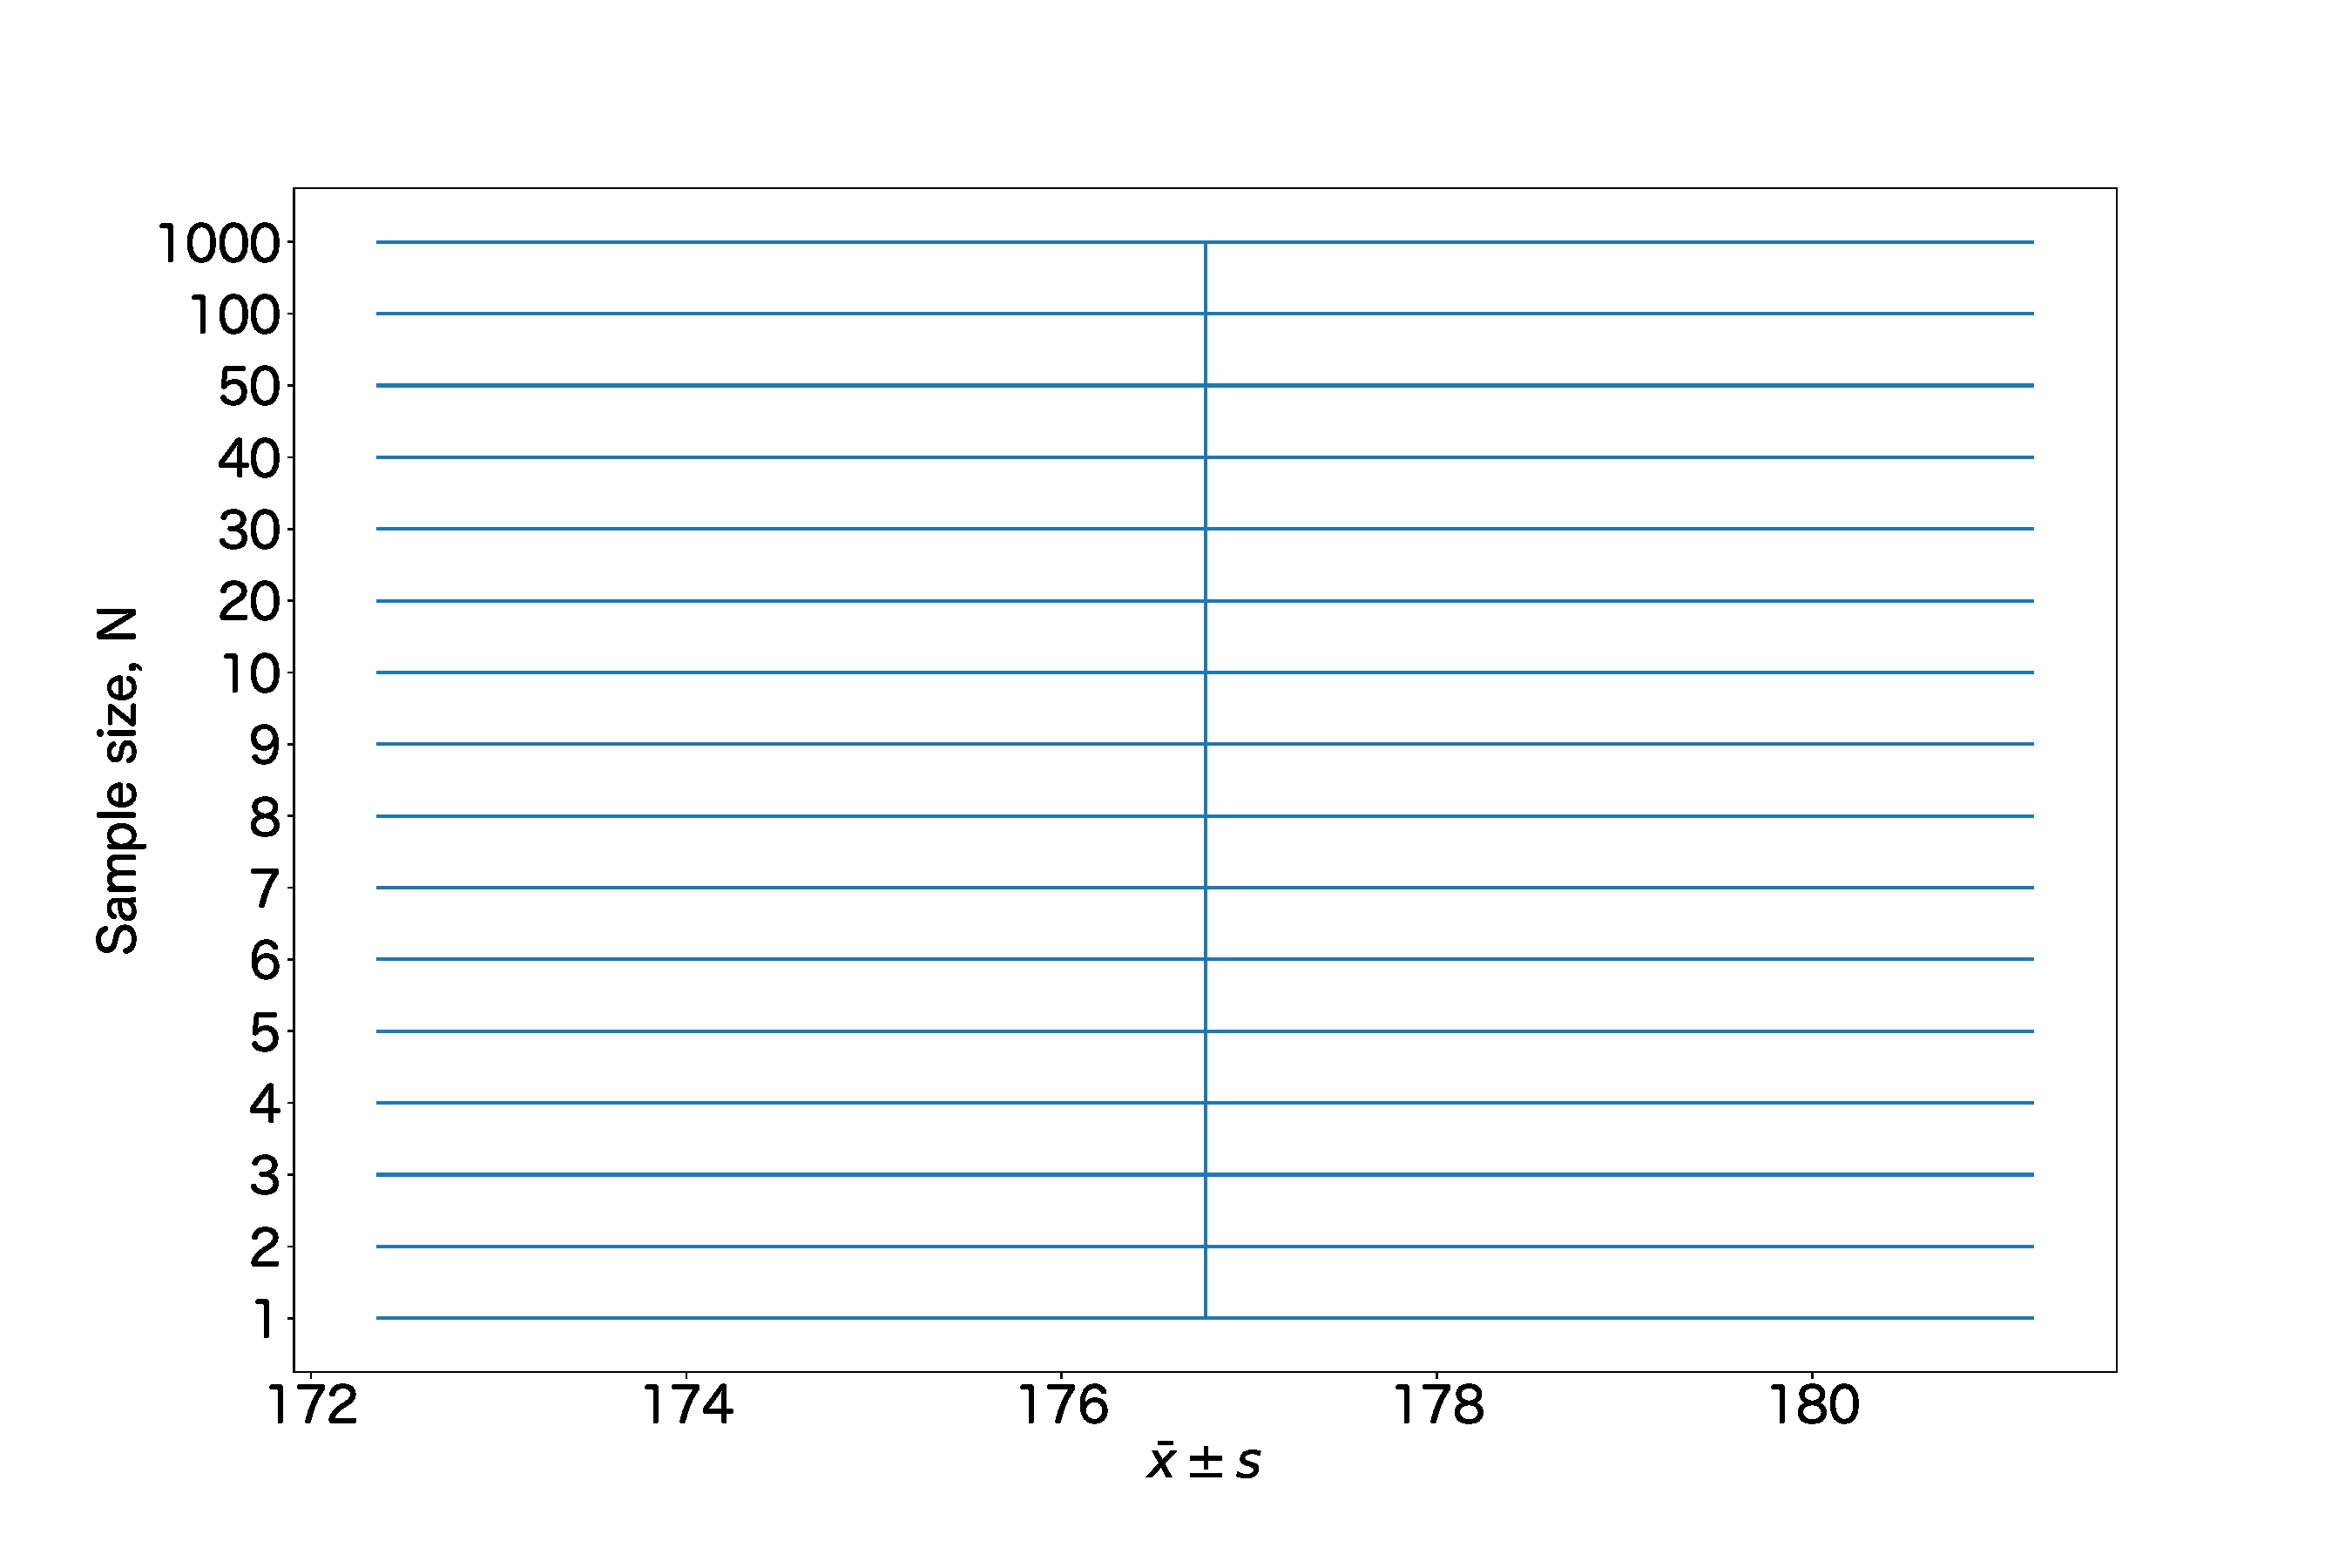
\includegraphics[width=15cm]{../markdown/section1/Norm_standard_deviation.pdf}
        \caption{サンプルサイズに応じた標準誤差の広がり}
        %\label{fig:standard_normal_distribution}
    \end{center}
\end{figure}



\subsubsection{標準誤差}
標準誤差$SE$は、標準偏差$s$をサンプルサイズ$N$の平方根で割ったものである。
\begin{equation*}
    SE = \frac{s}{\sqrt{N}}
\end{equation*}
$\bar{x}\sim N(\mu,\sigma^2/\sqrt(N))$であるので、モデルの上で$\bar{x}$が以下の範囲に出現する確率は、およそ$68.2\%$である。
\begin{equation*}
    [\bar{\mu}-SE,\bar{\mu}+SE]
\end{equation*}
よって、$\mu$の値は一般にわからないので、標本平均$\bar{X}$を用いて、
\begin{equation*}
    [\bar{X}-SE,\bar{X}+SE]
\end{equation*}
である。
統計モデル$M(\bar{x},s^2)$からサンプリングした$\bar{X}$がこの範囲に得られる確率が$68.2\%$である\footnote{$\sigma$が変曲点であるから使ったと思われるが、なぜ、$68.2\%$または、$\bar{X}\pm SE$の範囲を使ったのかはわからなかった。誤差論の立場では、以下の記述が見つかった\cite{誤差の取り扱い_神戸大学}。
\begin{quote}
    したがって、おおよそ$70\%$の確率で誤差の絶対値は$\sigma$より小さいことがわかるので、これを測定値の信頼度の目安として用いる。
\end{quote}
}
\footnote{標準偏差に ± を付けるな!: 医療論文に多い?
\url{https://biolab.sakura.ne.jp/mean-sd.html}。まだ読めていない。$\pm SE$という表記はよろしくないらしい。}。
言い換えれば、$SE$は、$68\%$信頼区間である。


\begin{figure}
    \begin{center}
        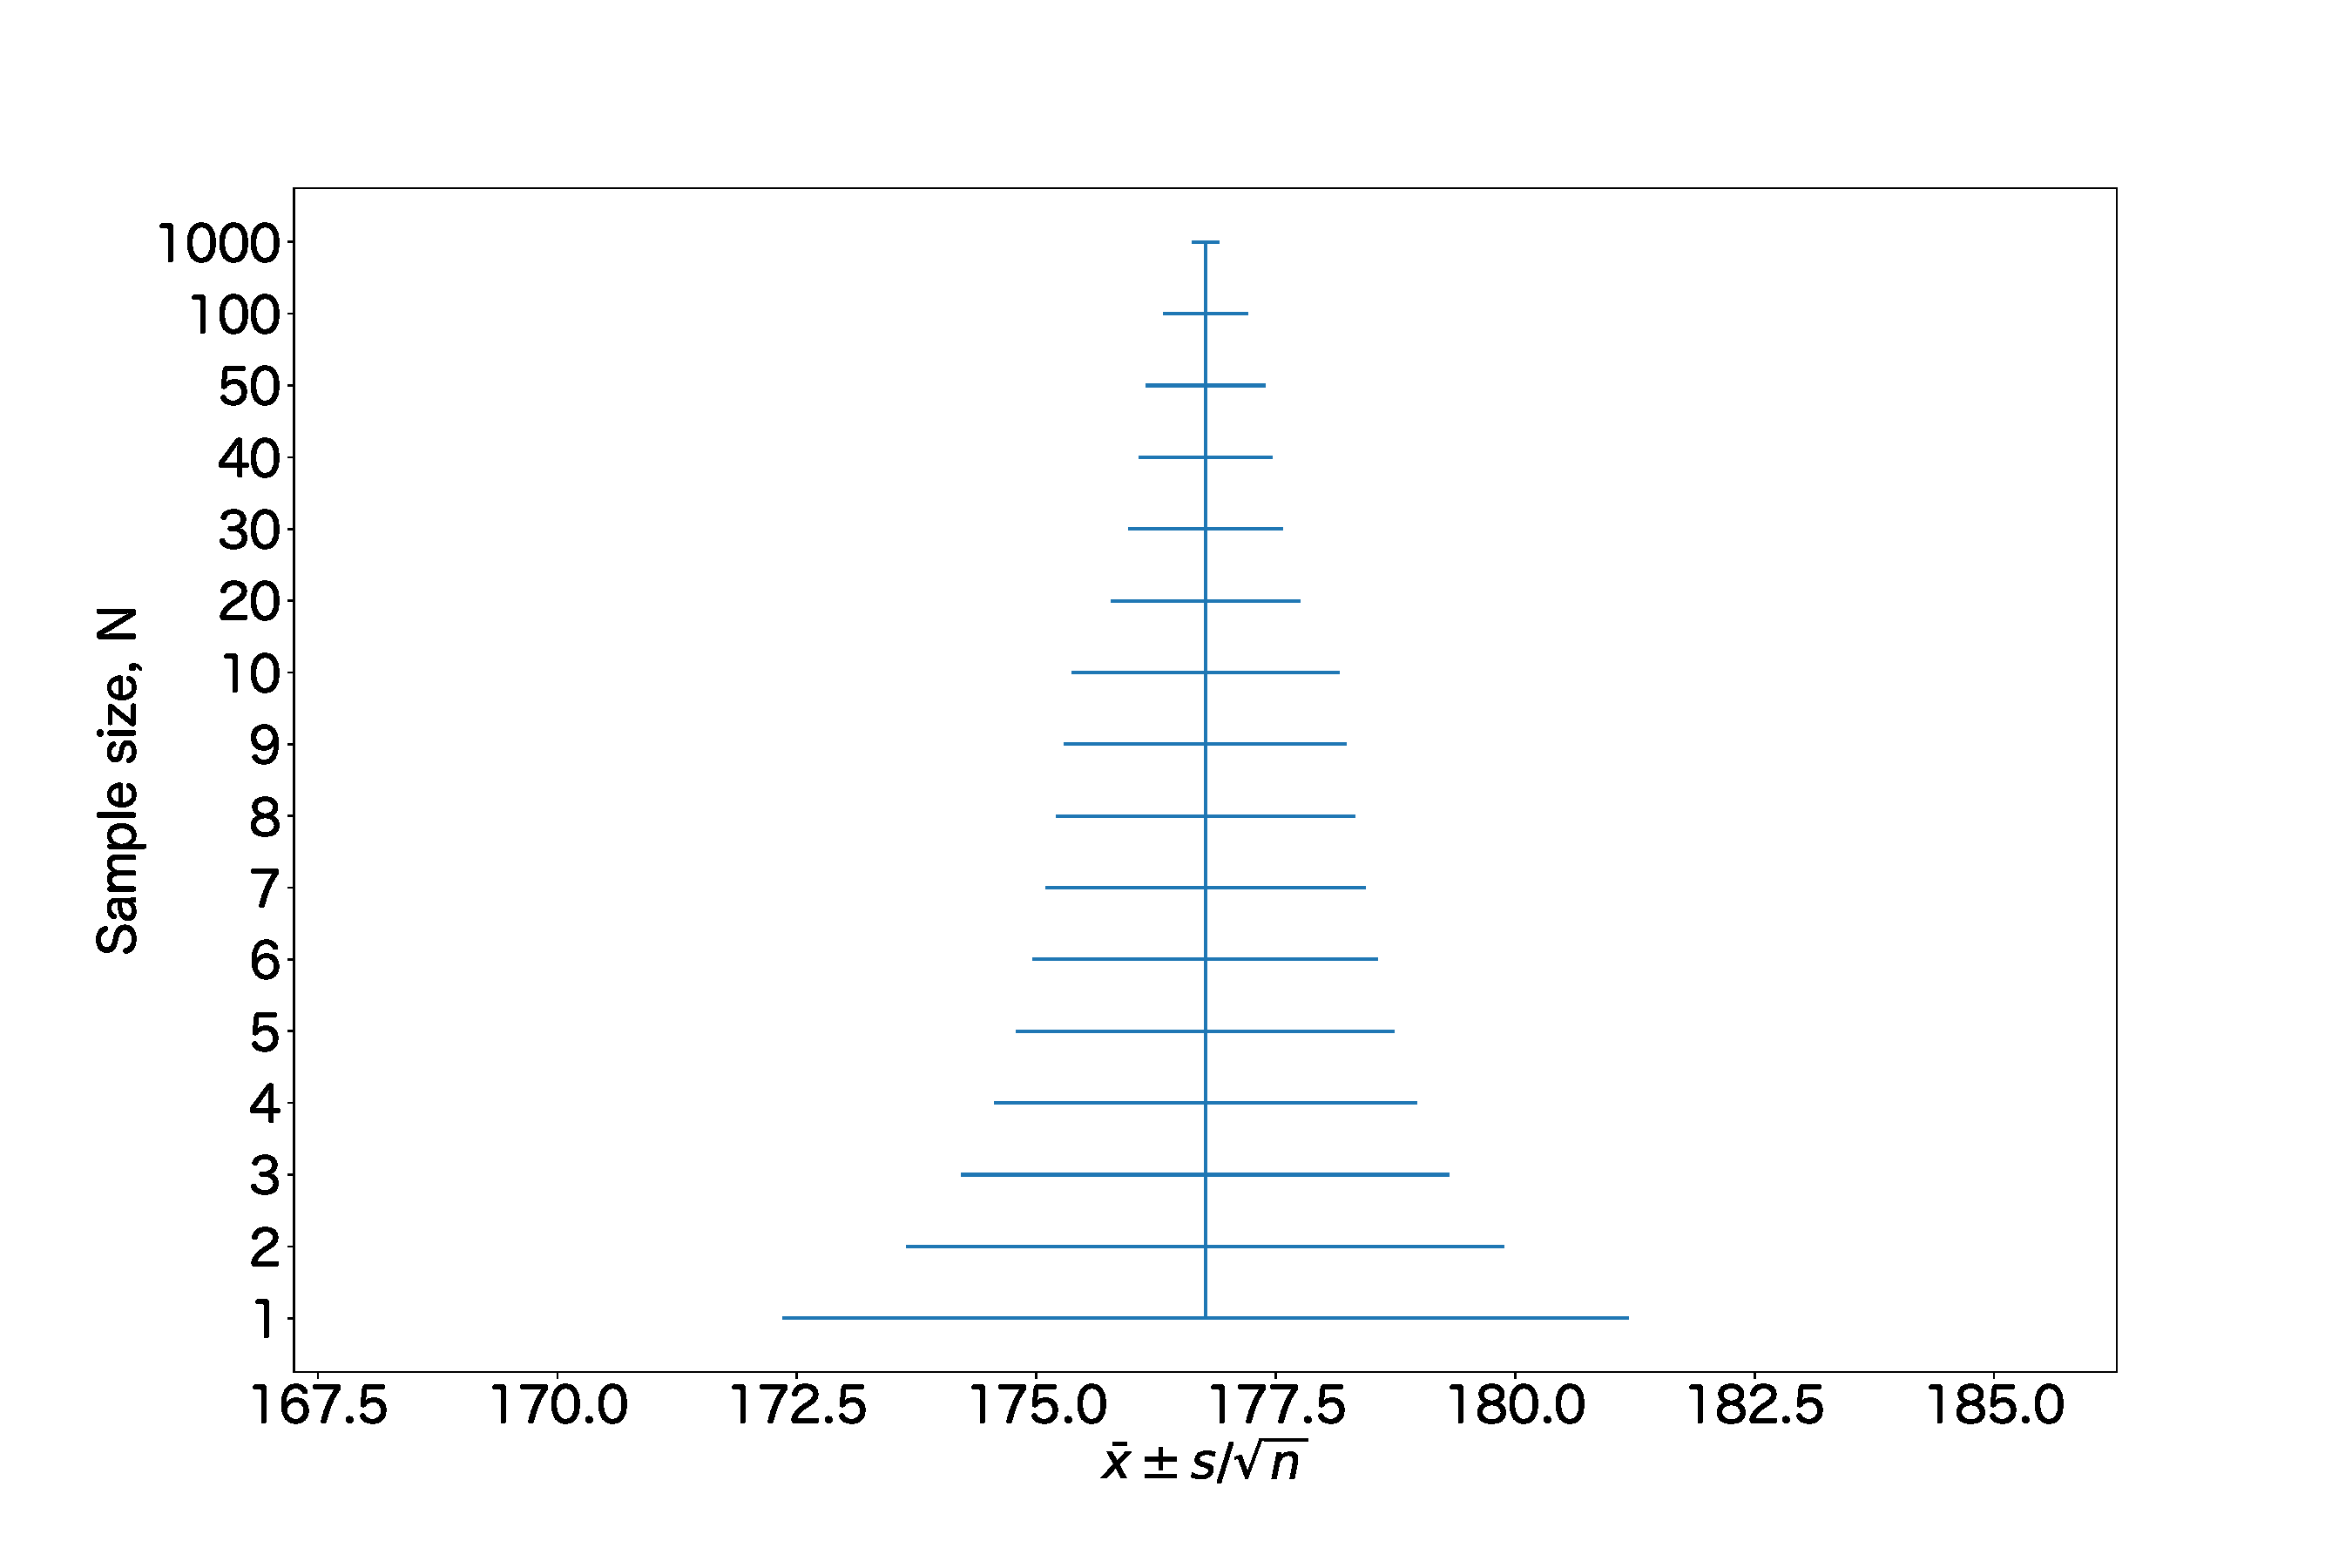
\includegraphics[width=15cm]{../markdown/section1/Norm_SE.pdf}
        \caption{サンプルサイズに応じた標準偏差の広がり}
        %\label{fig:standard_normal_distribution}
    \end{center}
\end{figure}

